\documentclass{article}
%% Useful packages
\usepackage[utf8]{inputenc}
\usepackage[a4paper,left=3.5cm,right=3.5cm,top=2cm,bottom=2cm]{geometry}
\usepackage{crop,graphicx,amsmath,array,color,amssymb,fancyhdr,lineno}
\usepackage{flushend,stfloats,amsthm,chngpage,times,,lipsum,lastpage} 
\usepackage{calc,listings,color,wrapfig,tabularx,longtable,enumitem}
\usepackage{multirow}
\usepackage{caption}
\usepackage{subcaption}
\usepackage{xcolor}
\usepackage{tcolorbox}
\definecolor{shadecolor}{rgb}{0.86,0.86,0.86}
\usepackage{float}

\usepackage{lineno}
\usepackage{csquotes}
\usepackage[italian]{babel}
%%%%%%%%%%%%   Header and Footer  %%%%%%%%%%%%%

\pagestyle{fancy}
\fancypagestyle{plain}{%
  \renewcommand{\headrulewidth}{0pt}%
  \fancyhf{}%
}

\title{%
        Creazione e confronto di Alberi Binari di Ricerca (ABR), Alberi Rosso-Neri (RB), Alberi AVL}
\author{Biondi Simone}

\begin{document}
\include{Title/title.tex}

\fancyhf{}
\fancyhead[L]{Simone Biondi}
\fancyhead[R]{Laboratorio di Algoritmi e Strutture Dati}
\fancyfoot[R]{ \large \bf \thepage\ \centering}%

\newpage
\tableofcontents
\newpage

\section{Introduzione Generale}
L'esercizio assegnatomi per il completamento del corso di Laboratorio di Algortimi e Strutture Dati viene riportato come segue:
\begin{itemize}
	\item {\textit  {"Vogliamo confrontare vari modi per costruire alberi di ricerca: normali ABR, alberi Rosso-Neri, alberi AVL."}}
\end{itemize}
	Nel paragrafo sottostante verranno elencati i punti salienti della intera relazione.

\subsection{Cosa affronterò}

Si può suddividere la relazione in 4 macro sezioni:

\begin{itemize}
	\item \textbf {Teoria e Problema}: in questa sezione affronterò l'esercizio da risolvere sfruttando la teoria appresa durante il corso di Algoritmi e Strutture Dati. Si descriverà brevemente le strutture dati che verranno utilizzate, gli algoritmi usati su tali strutture ed i risultati attesi (secondo la teoria) che verranno poi messi a confronto con quelli sperimentali.
	\item \textbf{Documentazione del codice}: in questa sezione descriverò come il codice python è stato implementato.
	\item \textbf{Descrizione degli esperimenti}: in questa sezione descriverò i risultati sperimentali ottenuti con grafici e tabelle.
	\item \textbf{Analisi dei risultati sperimentali}: in questa sezione esporrò una analisi critica di tutti i risultati ottenuti effettuando così le mie conclusioni.
\end{itemize}

\subsection{Calcolatore e Ambienti}
Di seguito vengono riportate le specifiche del Calcolatore utilizzato per il conseguimento dei test sperimentali; ambienti e linguaggio usati per la stesura del programma e della relazione stessa.

\begin{itemize}
	\item \textbf{Specs del Calcolatore}:
		\begin{itemize}
			\item \textbf{CPU}: Chip Apple M1, 8-core
			\item \textbf{RAM}: 8 GB
			\item \textbf{SSD}: 512 GB
		\end{itemize}
	\item \textbf{Linguaggio di Programmazione}: Python
	\item \textbf{Ambienti}: VS-Code, TexStudio
\end{itemize}
\section{Teoria e Problema}
\label{sezione2}
\subsection{Introduzione}
Per poter svolgere l'esercizio è necessario capire, anche se brevemente, cosa sono gli Alberi Binari di Ricerca (in generale) e successivamente una comprensione delle sue varianti più "potenti". 
In particolare come tali alberi sono visti come una Struttura Dati e conseguentemente gli eventuali Algoritmi che possono essere utilizzati su di essi.
L'Algoritmo su cui mi soffermerò in maniera approfondita sarà l'algoritmo di inserimento (per ogni tipologia di Albero Binario di Ricerca), in quanto essenziale per la loro creazione, e la sua complessità computazionale. Verrà fatto invece solo un accenno sulla complessità computazionale della ricerca e della cancellazione (senza approfondimento).
\subsection{Notazioni e concetti da usare}
Per trattare i successivi argomenti è necessario usufruire di alcune notazioni della teoria della complessità computazionale, come ad esempio $O(\cdot)$ e $\Theta(\cdot)$. Infine faremo riferimento a \textit{n} come al numero di nodi di un albero ed \textit{h} come la sua altezza. Infine useremo $lg(n)$ = $\log_{2}(n)$ come notazione per il logaritmo in base 2.
\subsection{Cosa è un Albero Binario di Ricerca?}
Gli Alberi Binari di Ricerca (brevemente ABR) sono strutture dati che supportano molte operazioni sugli insiemi dinamici. Gli ABR sono organizzati in alberi binari dove ogni Nodo è visto come un oggetto. Ciascun Nodo possiede pertanto i seguenti campi:
\begin{itemize}
	\item \textit{Key}: la chiave, valore, del nodo in questione più eventuali dati satelliti
	\item \textit{Left}: puntatore al figlio sinistro
	\item \textit{Right}: puntatore al figlio destro
	\item \textit{p}: puntantore al padre.
\end{itemize}
Se manca un figlio o un padre i corrispondenti campi hanno valore \textbf{NIL}. Il nodo Radice \textit{(Root)} è l'unico nodo il cui campo padre \textit{p} è \textbf{NIL}.
\subsection{Proprietà fondamentale di un ABR}
Le chiavi in un ABR sono memorizzate sempre in modo tale da soddisfare la \textbf{\textit{Proprietà fondamentale di un ABR}}:
\begin{tcolorbox} [colback=lightgray!20,%gray background
colframe=black,% black frame colour
arc=3mm, auto outer arc,]
	\textit{Sia x un nodo all'interno di un ABR. Allora:
		\begin{itemize}
			\item se y è un nodo nel sottoalbero sinistro di x allora y.key $<$ x.key
			\item se y è un nodo nel sottoalbero destro di x, allora y.key $\geq$ x.key
		\end{itemize}}
\end{tcolorbox}
Un esempio grafico che rispetti tale proprietà è il seguente:
\begin{figure}[H]
	\centering
	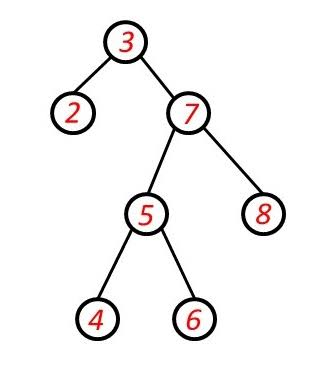
\includegraphics[width=0.3\textwidth]{Resources/ABR_Esempio.jpeg}
	\caption{Esempio di ABR generico}
	\label{fig:immagine}
\end{figure}

\subsection{Altezza di un ABR e Algoritmi Base}
Un fattore molto importante di un ABR, in quanto è una struttura ad albero, è la sua \textbf{altezza}.
 Il costo computazionale per ogni algoritmo utilizzato su tale struttura dati sono determinati da essa.
Algoritmi che di base vengono utilizzati sugli ABR per la manipolazione dei dati sono:
\begin{itemize}
	\item \textbf{Inserimento}
	\item \textbf{Ricerca}
	\item \textbf{Cancellazione}
\end{itemize}
\subsubsection{Inserimento}
L'inserimento di un nodo all'interno dell'ABR viene fatto sfruttando a pieno la proprietà fondamentale di un ABR. Sia pertanto \textit{x} il nodo corrente e sia \textit{z} il nodo da inserire:
\begin{itemize}
	\item la chiave del nodo \textit{z} viene confrontata con la chiave del nodo corrente \textit{x};
	\item in base a tale confronto navigo all'interno dell'albero o a sinistra oppure a destra (in base all'esito del confronto);
	\item la navigazione termina quando \textit{x=NIL}, ovvero sia \textit{x} punta ad una Foglia dell'albero.
\end{itemize}
\subsubsection{Ricerca e Cancellazione}
Ai fini della relazione tratterò solamente i Costi Computazionali a confronto con AVL e RB per la ricerca e cancellazione. Non mi soffermo, in questa sezione, sugli algoritmi di tali metodi.
\subsection{Costo Computazionale}
Per un albero ABR generale la complessità computazionale di un algoritmo di Ricerca, Inserimento o Cancellazione è $\mathcal{O}(h)$ , dove $h$ è l'altezza dell'albero.
Nel caso medio, assumendo che le chiavi siano inserite in ordine
casuale, l'altezza attesa dell'ABR è $\Theta(lg(n))$.
Si distinguono però per l'\textbf{Inserimento} due casi particolari molto importanti:
\begin{itemize}
	\item \textbf{Caso Migliore}: in questa situazione l'altezza dell'albero è circa $\Theta(lg(n))$. Difatti considerando l'albero con questa altezza, per un nodo da inserire, l'inserimento ha complessità computazionale di $\mathcal{O}(\lg(n))$. Questo perchè il confronto della chiave del nodo da inserire non viene fatto con tutti i nodi già presenti all'interno dell'albero in quanto l'albero stesso è "bilanciato" (ovvero sia l'albero presenta in maniera "più o meno simile" il numero di nodi sia a destra che a sinistra prendendo un qualunque nodo come riferimento);
	\item \textbf{Caso Peggiore}: l'albero degenera in una lista. In questa situazione l'altezza dell'albero è circa $\Theta(n)$. Questo avviene quando si ha un inserimento "contiguo" o tutto a sinistra o tutto a destra dell'albero, ovvero sia quando l'inserimento avviene per valori in ordine crescente o decrescente. In questo caso il costo per un singolo inserimento è pari a $\mathcal{O}(n)$.
\end{itemize}
Si ricorda che per un ABR generico, senza proprietà aggiunte, non è presente un ribilanciamento dell'albero.
\subsection{RB e AVL}
Come anticipato esistono delle varianti più potenti di ABR: gli AVL e i RB. Sono varianti che introducono delle proprietà nuove che permettono all'albero un ribilanciamento (in base alle specifiche proprietà) che permettono di abbattere i costi computazionali e di evitare una degenerazione come nel caso dell'inserimento per un ABR generico. Vediamo quindi brevemente le nuove proprietà introdotte e come le due tipologie di varianti riescono a gestire, in particolare per l'inserimento, un ribilanciamento dell'albero binario di ricerca con il fine di abbassare la complessità computazionale.
Per entrambe le varianti si introducono \textbf{Algoritmi di Rotazione Left/Right}, utili per ribilanciare la struttura (più ricolorazioni per gli alberi Rosso-Neri).
\subsubsection{AVL}
Un albero AVL è un albero ABR che si mantiene bilanciato dopo gli inserimenti (e cancellazioni). La proprietà aggiuntiva che viene introdotta è la seguente: 
\begin{tcolorbox} [colback=lightgray!20,%gray background
	colframe=black,% black frame colour
	arc=3mm, auto outer arc,]
	\centering{\textit{Per ogni nodo dell'albero vale} $|h_{sinistro} - h_{destro}| \leq 1$}
\end{tcolorbox}
La nuova regola introdotta ci dice che, in ogni nodo, l'altezza del sottoalbero sinistro e destro può differire al massimo di 1. Se tale proprietà viene violata, l'AVL esegue rotazioni per ribilanciare localmente la struttura. Questo ci garantisce che l'altezza dell'albero è $\Theta(\lg(n))$ e pertanto inserimento, ricerca e cancellazione hanno un costo $\mathcal{O}(\lg(n))$. Si deduce appunto che il caso peggiore visto da un ABR generico viene tranquillamente risolto tramite gli AVL.
\subsubsection{RB}
Un albero Rosso-Nero (\texttt{Red-Black [RB]}) è un ABR auto-bilanciato: per ogni nodo si introduce un colore che può essere rosso oppure nero. Le principali (e quindi nuove) proprietà introdotte sono:
\begin{itemize}
	\item La radice è nera.
	\item Le foglie \textbf{NIL} sono nere.
	\item Un nodo rosso non può avere figli rossi.
	\item Ogni cammino da un nodo a una foglia \textbf{NIL} contiene il medesimo numero di nodi neri.
\end{itemize}
Con queste nuove proprietà si impedisce che l'albero diventi troppo sbilanciato e pertanto dopo inserimenti o cancellazioni, vengono usate ricolorazione dei nodi e rotazioni per ribilanciare localmente la struttura. Come gli AVL, i RB garantiscono altezza $\Theta(lg(n))$ e pertanto per metodi di inserimento e cancellazione il costo computazionale è $\mathcal{O}(lg(n))$. Come nel caso precedente si deduce che il caso peggiore visto da un ABR generico viene tranquillamente risolto anche tramite i RB.
\subsection{Una prima conclusione: assunti ed ipotesi}
\label{Sezione2.8}
Nella \hyperref[sezione2]{Sezione 2} abbiamo affrontato la parte teorica per fare fronte agli esperimenti condotti. Per gli esperimenti affronteremo due casi particolari di costruzioni di alberi binari di ricerca e sue varianti come segue:
\begin{itemize}
	\item \textbf{Caso 1:}  Vengono inserite chiavi distinte in un ordine
	casuale [\textit{Caso medio}]
	\item \textbf{Caso 2:} Vengono inserite chiavi distinte in ordine
	strettamente crescente (o decrescente). L'ABR generico degenera,
	mentre AVL e RB mantengono il bilanciamento [\textit{Caso peggiore per ABR generico}].
\end{itemize}
Le \hyperref[Tabelle2.9]{Tabelle in 2.9} ci permettono di avere un primo confronto tra le diverse strutture dati usate e come l'algoritmo dell'Inserimento si distingue, in termini di costi computazionali, tra le 3 tipologie di ABR per entrambe le casistiche. L'obbiettivo è pertanto quello di verificare che i risultati attesi delle complessità computazionali siano veritieri attraverso la sperimentazione.
\subsection{Tabella delle complessità computazionali a confronto}
Le tabelle seguenti presentano i risultati attesi da verificare successivamente sperimentalmente: ricerca e cancellazione sono riportate come confronto teorico (un approfondimento verrà fatto nella \hyperref[Sezione5.2]{Sezione 5.2}); la sperimentazione considera solamente il costo di costruzione mediante l'inserimento. Per ciascuno dei 2 esperimenti verranno introdotti \textit{x} nodi, sia per il caso randomico e sia per il caso peggiore. Riportiamo in ogni caso il costo computazionale per una singola operazione tra inserimento, ricerca e cancellazione. Si faccia riferimento alla \hyperref[Sezione2.8]{Sezione 2.8} per "Caso 1" e "Caso 2":
\label{Tabelle2.9}
\begin{figure}[H]
	\centering
	\begin{tabular}{|c|c|c|}
		\hline
		& Caso 1 & Caso 2\\
		\hline
		\textcolor{blue}{Inserimento} & $O(lg(n))$ & $O(n)$\\
		\hline
		Ricerca & $O(lg(n))$ & $O(n)$\\
		\hline
		Cancellazione & $O(lg(n))$ & $O(n)$\\
		\hline
	\end{tabular}
	\caption{Complessità degli algoritmi di ABR}
	\label{fig:ComplessitàABR}
\end{figure}

\begin{figure}[H]
	\centering
	\begin{tabular}{|c|c|c|}
		\hline
		& Caso 1 & Caso 2\\
		\hline
		\textcolor{blue}{Inserimento} & $O(lg(n))$ & $O(lg(n))$\\
		\hline
		Ricerca & $O(lg(n))$ & $O(lg(n))$\\
		\hline
		Cancellazione & $O(lg(n))$ & $O(lg(n))$\\
		\hline
	\end{tabular}
	\caption{Complessità degli algoritmi di AVL e RB}
	\label{fig:ComplessitàAVL}
\end{figure}
\section{Documentazione del codice}
\subsection{Strutture Dati}
Ciascuna struttura dati si ritrova all'interno del file \texttt{strutture\_dati.py}.
Le strutture dati implementate nel codice per ogni tipo di albero binario di ricerca sono le seguenti (ciascuna struttura è da considerarsi una classe):
\begin{itemize}
	\item \textbf{AlberoABR}
	\item \textbf{AlberoAVL}
	\item \textbf{AlberoRB}
	\item \textbf{Foglia}
	\item \textbf{Nodo\_ABR}
	\item \textbf{Nodo\_AVL}
	\item \textbf{Nodo\_RB}
\end{itemize}
Le classi \texttt{AlberoABR}, \texttt{AlberoAVL}, \texttt{AlberoRB} sono le classi che descrivono appunto l'albero binario di ricerca, l'albero AVL e l'albero RB.
La classe \texttt{Foglia} rappresenta il nodo sentinella \texttt{NIL},
utilizzato nelle implementazioni AVL e Rosso-Neri per rappresentare
l'assenza di nodi-figli.
Infine per ciascun tipo di albero binario di ricerca è stata fatta una classe a sè stante per ogni "tipologia" di nodo.
\subsection{Metodi}
I principali metodi che sono stati utilizzati all'interno del programma si ritrovano, come suggeriscono i nomi stessi, all'interno di ciascuna classe per ogni tipologia di albero. Essi sono i seguenti:
\begin{itemize}
	\item \textbf{Inserimento}: una volta inizializzata ciascuna tipologia di albero, si prosegue ad inserire gli eventuali nodi (sia per il caso 1 che per il caso 2). I metodi richiamano, nella loro denominazione, a quale tipo di albero fanno riferimento. Abbiamo per cui \texttt{ABR\_Tree\_Insert(z)}, \texttt{AVL\_Tree\_Insert(z)}, \texttt{RB\_Tree\_Insert(z)}. Quando il metodo viene invocato, il riferimento all'albero viene effettuato tramite \texttt{self}; $z$ è invece il nodo che viene inserito all'interno dell'albero;
	\item \textbf{Fix-Up}: I metodi di fix-up sono presenti solamente nelle implementazioni AVL e RB. Dopo un inserimento, essi risalgono il cammino dal nodo modificato verso la radice e ripristinano le proprietà di bilanciamento mediante aggiornamenti delle altezze, rotazioni e, nel caso RB, ricolorazioni. Troviamo pertanto \texttt{RB\_Insert\_Fixup(z)} e \texttt{AVL\_Insert\_Fixup(z)}. Il nodo $z$ viene distinto dal tipo di albero in esame ossia per gli AVL è il padre del nodo appena inserito; per gli alberi RB invece è il nodo che è stato appena inserito;
	\item \textbf{Rotazioni}: i metodi di Fix-up richiamano a loro volta i metodi delle Rotazioni in quanto, come detto, alberi AVL e RB usufruiscono delle rotazioni per poter ribilanciare localmente l'albero e non far violare le loro proprietà. Pertanto abbiamo \texttt{AVL\_Left\_Rotate(x)}, \texttt{AVL\_Right\_Rotate(x)}, \texttt{RB\_Left\_Rotate(x)}, \texttt{RB\_Right\_Rotate(x)}. Per ciascun metodo si ha un riferimento all'albero stesso tramite \texttt{self}, mentre $x$ è il nodo dove verrà applicata la rotazione.
\end{itemize}
\subsection{Note sul programma principale: \texttt{main.py}}
Per il programma principale sono state utilizzate librerie di Python in modo tale da:
\begin{itemize}
	\item poter generare, ai fini dell'esperimento, grafici di confronto [\texttt{matplotlib.pyplot}];
	\item misurare il tempo di esecuzione [\texttt{time}];
	\item generare valori casuali per trattare il caso casuale, corrispondente al caso medio [\texttt{random}];
	\item liberare la memoria tramite l'uso del garbage-collector [\texttt{gc}].
\end{itemize}
Sempre all'interno di \texttt{main.py}, per poter garantire la riproducibilità del caso medio, è stato fissato il $seed$ del generatore casuale al valore $42$. Conseguentemente, ad ogni esecuzione, le tre strutture ricevono la medesima permutazione casuale delle chiavi.
Inoltre il programma è stato suddiviso, sia per il caso 1 che per il caso 2 (si faccia riferimento alla sezione 2.8), in 3 parti. Pertanto si considera ciascuna azione sottostante ripetuta 2 volte:
\begin{itemize}
	\item \textbf{Inizializzazione}: ogni Albero sotto esame viene inizializzato istanziandone la classe. Vengono aggiunti 2 array per ciascun tipo di albero i quali contengono, rispettivamente, i nodi inseriti e i tempi di inserimento per ogni nodo;
	\item \textbf{Inserimento}: attraverso un parametro detto \texttt{MAX\_NODI} è possibile scegliere il numero di nodi da poter inserire all'interno di ciascun albero sia per il caso 1 che per il caso 2. Si approfondirà l'argomento nella sezione 4;
	\item \textbf{Grafici}: per entrambi i casi verranno disposti 2 grafici contenti i risultati ottenuti tramite gli inserimenti. In particolare avremmo, per ogni grafico, i tempi cumulativi di inserimento lungo le ordinate (ossia viene registrato il tempo cumulativo necessario a costruire l'albero fino a $x$ nodi) mentre lungo le ascisse avremmo il numero di nodi inseriti. Questo ci permette di poter ottenere un confronto visivo e di poter quindi constatare la teoria trattata nella sezione 2.
\end{itemize}
Una ulteriore nota, di molta importanza, fa riferimento al parametro \texttt{LIMITE}. Questo parametro è stato introdotto in quanto l'inserimento per il caso 2 poteva richiedere un grande quantitativo di tempo per poter terminare (con particolare attenzione ad un ABR generico). Questa situazione si aggravava con l'aumentare del parametro \texttt{MAX\_NODI} e pertanto la soluzione è stata quella di introdurre un limite temporale.\\ 
Questo dettaglio verrà comunque riaccennato nella sezione 4.\\ \\
Infine il \textbf{Terminale}, tramite righe di codice, permette di poter visualizzare testualmente l'andamento del programma in modo tale da tenere traccia di cosa sta succedendo prima della generazione dei grafici di confronto finali.
\subsection{Diagramma delle classi}
A seguire il diagramma delle classi: 
\begin{figure}[H]
	\centering
	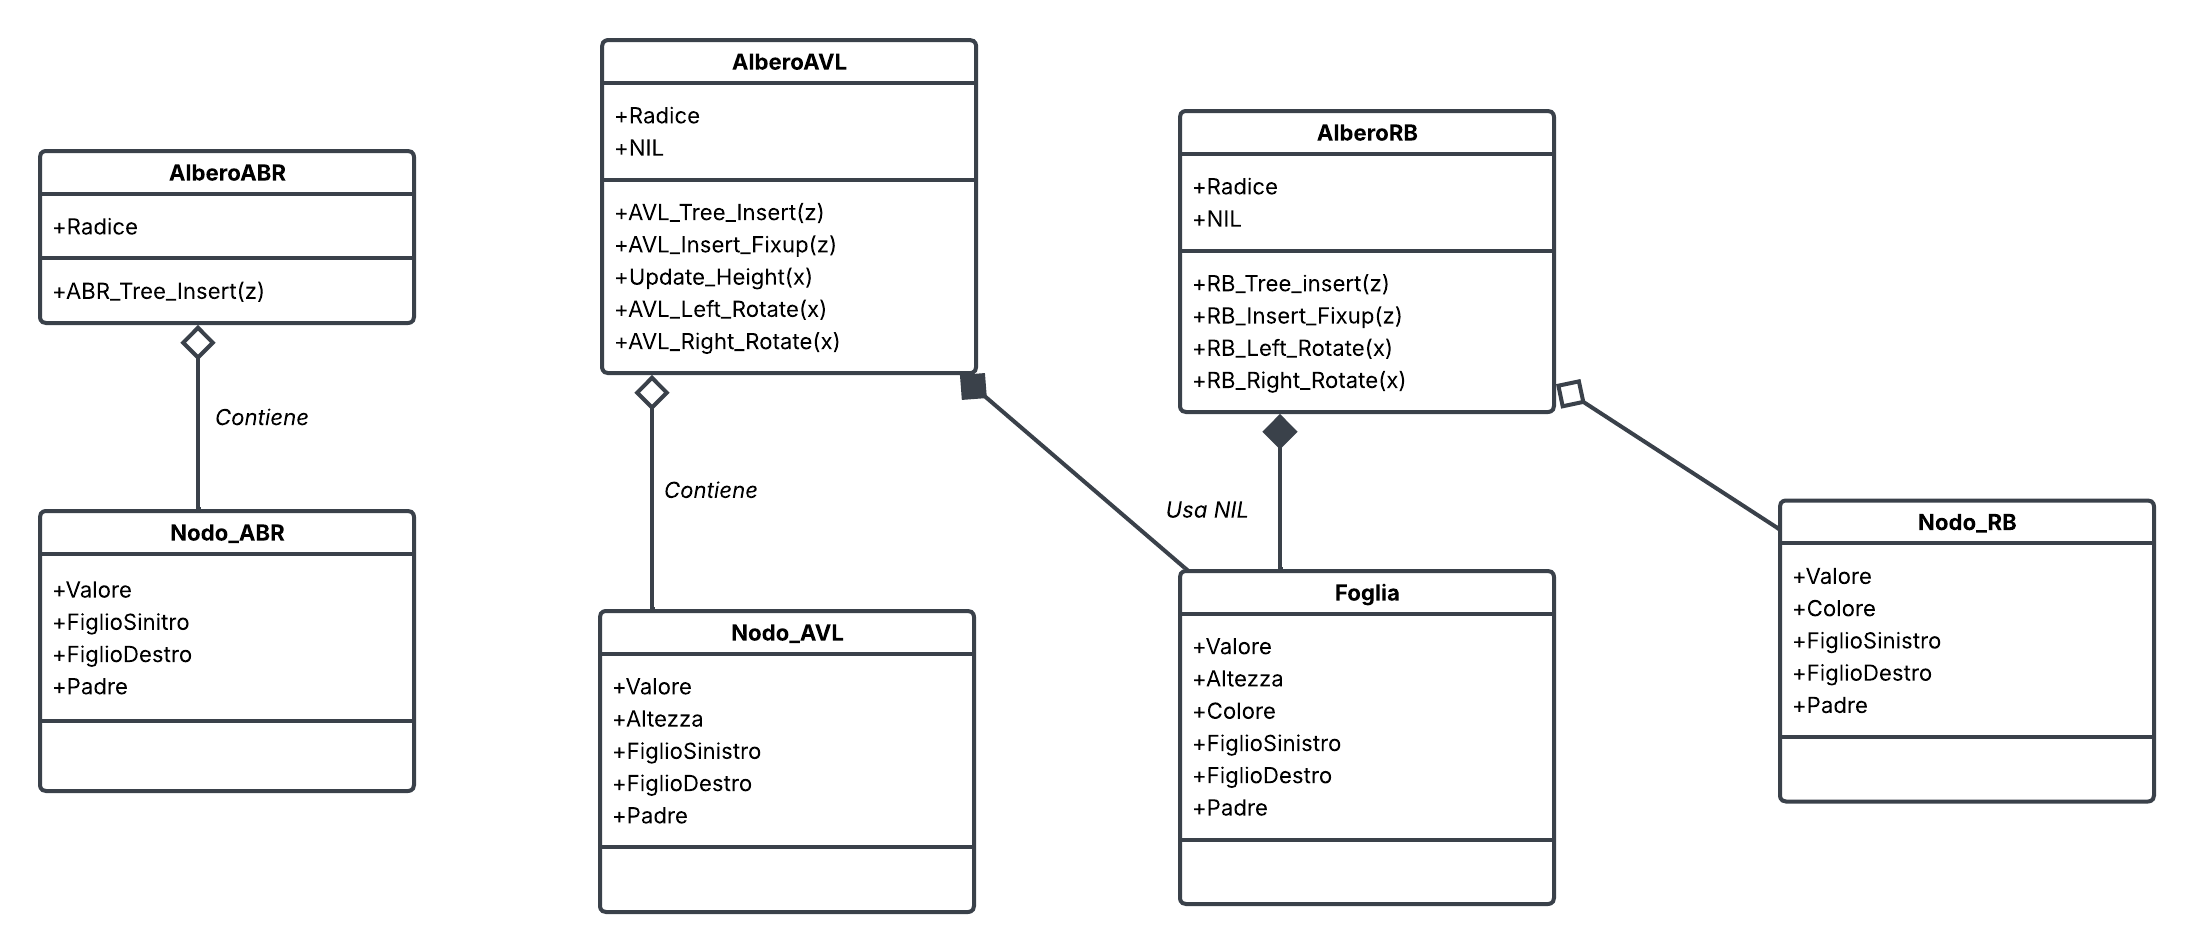
\includegraphics[width=0.9\textwidth]{Resources/UML2.png}
	\caption{Diagramma delle Classi}
	\label{fig:img}
\end{figure}
Il diagramma mostra le tre strutture principali:
\begin{itemize}
	\item \textbf{AlberoABR} contiene nodi di tipo \textbf{Nodo\_ABR};
	\item \textbf{AlberoAVL} contiene nodi di tipo \textbf{Nodo\_AVL} e usa una foglia sentinella \textbf{NIL} rappresentato dalla classe \textbf{Foglia};
	\item \textbf{AlberoRB} contiene nodi di tipo \textbf{Nodo\_RB} e usa anch'esso una foglia sentinella \textbf{NIL} della classe \textbf{Foglia}.
\end{itemize}
Le classi di "tipo" \texttt{Nodo\_X} rappresentano i singoli nodi degli alberi. Tutte possiedono attributi \texttt{Valore, FiglioSinistro, FiglioDestro, Padre}. Per nodi di tipo AVL è stato aggiunta \texttt{Altezza}, mentre per nodi di tipo RB è stato aggiunto \texttt{Colore}.
Non ci sono relazioni di ereditarietà in quanto ogni tipo di albero e ogni tipo di nodo sono implementati in classe separate. I metodi principali sono dentro le rispettive classi (in aggiunta è stato messo anche il metodo [\texttt{Update\_Height(x)}] per l'aggiornamento dell'altezza del nodo $x$ in riferimento all'albero AVL).
Infine, tramite la simbologia usata per diagrammi UML, abbiamo:
\begin{itemize}
	\item -$\lozenge$: l'albero contiene nodi;
	\item -$\blacklozenge$: l'albiero possiede il nodo sentinella \texttt{NIL}.
\end{itemize}

\section{Descrizione ed Analisi dei risultati sperimentali}
\label{Sezione4}
\subsection{Cosa ci dobbiamo aspettare}
Come anticipato nelle sezioni precedenti, in particolare in riferimento alla 2.8, la descrizione degli esperimenti verterà su due casistiche particolari con lo scopo di vedere come un albero binario di ricerca venga creato e, ai fini della relazione, confrontare i risultati sperimentali con la teoria (e quindi con risultati attesi) vista fino ad ora.
L'obbiettivo è pertanto quello di verificare i costi computazionali nella creazione di un ABR generico, di un AVL e di un RB per i casi 1 e 2 (2.8) e confrontare tali risultati con la teoria. Da ora considereremo per qualunque tipo di casistica l'inserimento di $n$ nodi.\\ \\
Per il \textbf{caso medio} ci aspettiamo che il costo di una singola inserzione per ABR, AVL e RB è  $\mathcal{O}(lg(n))$. Poichè i grafici misurano il tempo cumulativo di costruzione dopo $n$ inserimenti, ci aspettiamo un andamento $\Theta(nlgn)$, che nell'intervallo sperimentale considerato appare quasi lineare.
\begin{tcolorbox}[colback=lightgray!20,%gray background
	colframe=black,% black frame colour
	arc=3mm, auto outer arc,] \textbf{Attenzione:} dovremmo prestare particolare attenzione alle costanti che possono entrare in gioco. Ricordiamo dalla teoria della complessità computazionale che una scrittura del tipo $\mathcal{O}(f(n))$ sta a indicare un limite superiore asintotico al costo computazionale in funzione di $f(n)$. Nel caso medio, ABR, AVL e RB hanno lo stesso ordine di complessità,
	ma possono mostrare tempi sperimentali differenti. In particolare, ci
	si può aspettare che l'AVL presenti una costante moltiplicativa maggiore, poiché mantiene un bilanciamento più rigido. Infatti ad ogni inserimento, l'AVL:
	\label{CostoAVL}
	\begin{itemize}
		\item risale verso la radice;
		\item aggiorna l'attributo $altezza$ dei nodi;
		\item calcola la differenza (in modulo) di altezza tra figlio sinistro e figlio destro del nodo corrente;
		\item se necessario esegue una o due rotazioni.		
	\end{itemize}
	L'ABR, invece, individua la posizione corretta e collega il nuovo nodo
	senza aggiornare altezze o ribilanciare l'albero. Anche l'albero
	Rosso-Nero può eseguire ricolorazioni e rotazioni, ma il suo vincolo di
	bilanciamento è meno rigido rispetto a quello AVL e, in media, richiede
	meno rotazioni o aggiornamenti. \\
	Nell'ultima sezione dedicherò un paragrafo che tratta l'uso di AVL e RB a confronto ed eventuali vantaggi e svantaggi. \\
\end{tcolorbox}
Infine per il \textbf{caso peggiore}, quindi il "caso ordinato",  ci aspettiamo solamente una modifica al costo computazionale per gli ABR generici. Per un inserimento singolo abbiamo già visto che il costo per un ABR generico è di $\mathcal{O}(n)$: pertanto inserendo $n$ nodi ci aspettiamo un costo computazionale $\Theta(n^2)$; resta invece invariato per AVL e RB, ossia $\Theta(nlg(n))$.
\subsection{Misurare il tempo}
Ai fini dell'esperimento è stata utilizzata la libreria Python \texttt{time}, in particolare la funzione \texttt{perf\_counter()}.
Il tempo misurato è cumulativo: dopo l'inserimento dell'$n$-esimo nodo,
viene memorizzato il tempo trascorso dall'inizio della costruzione
dell'albero.
L'operazione di salvataggio nell'array può essere rappresentata come: \[
\texttt{tempi\_y}[n] =
t_{\mathrm{fine},n} - t_{\mathrm{inizio}}
\]
dove $y \in \{\mathrm{ABR}, \mathrm{AVL}, \mathrm{RB}\}$ identifica la
tipologia di albero.
Indicando con $t_y(i)$ il tempo necessario per inserire l'$i$-esimo
nodo nell'albero di tipo $y$, il tempo cumulativo dopo $n$ inserimenti è: \[
T_y(n) = \sum_{i=1}^{n} t_y(i)
\]
Pertanto poichè il tempo è cumulativo e non calcolato per ogni singola inserzione ci dobbiamo aspettare un andamento "quasi lineare" nel caso medio per tutte e 3 le tipologie di albero. Questo perchè una curva logaritmica cresce molto lentamente; per il caso peggiore invece ci dovrà essere una differenza sostanziale tra ABR generici contro AVL e RB.
\subsection{Input utilizzati}
\label{Sezione4.3}
Grazie al parametro \texttt{MAX\_NODI} presente in \texttt{main.py} possiamo analizzare diversi tipi di input per entrambe le casistiche. L'esperimento verterà su 3 diverse tipologie di input e quindi consideremo 3 casisistiche con un numero di nodi da inserire sempre più grande:
\begin{itemize}
	\item \textbf{5.000}: caso "base" che permette di cominciare ad avere una idea dei vari costi computazionali attesi;
	\item \textbf{50.000}: caso in cui la curva quadratica per il caso peggiore di ABR generico diventa sempre più evidente;
	\item \textbf{100.000}: caso in cui portiamo all'estremo l'esperimento.
\end{itemize}
\subsection{Alberi con 5.000 elementi}
In questa prima sezione vediamo come la costruzione delle 3 tipologie di albero si comportano a fronte di un numero di nodi in input "abbastanza basso":
\begin{figure}[H]
	\centering
	\includegraphics[width=0.7\textwidth]{Resources/figure_1.png}
	\caption{Caso Medio con 5.000 nodi}
\end{figure}
\begin{figure}[H]
	\centering
	\includegraphics[width=0.7\textwidth]{Resources/figure_2.png}
	\caption{Caso Peggiore con 5.000 nodi}
\end{figure}
Nella prima figura, come anticipato in 4.2, si può vedere un andamento "quasi lineare" per tutte e 3 le tipologie di albero.
Si può notare inoltre, come predetto in \hyperref[CostoAVL]{4.1}, che l'AVL presenta un costo computazionale leggermente più alto rispetto a ABR generici e RB: questo a causa del suo ribilanciamento più rigido. \\
Nella seconda figura invece, come ci aspettavamo, si intravede una curva quadratica per ABR generico; per RB e AVL invece si rispetta sempre l'andamento "quasi lineare".
\subsection{Alberi con 50.000 elementi}
In questa seconda sezione vediamo come la costruzione delle 3 tipologie di albero si comportano a fronte di un numero maggiore di nodi in input. In questo caso ha notevole importanza il parametro \texttt{LIMITE} presente in \texttt{main.py}. Questo perchè al crescere dell'input, l'ABR generico può impiegare molto più tempo durante l'inserimento a causa dell'elevato numero di confronti che deve fare. Tale limite temporale è stato settato a 30 secondi (ma può essere modificato a piacere):
\begin{figure}[H]
	\centering
	\includegraphics[width=0.8\textwidth]{Resources/figure_3.png}
	\caption{Caso Medio con 50.000 nodi}
\end{figure}
\begin{figure}[H]
	\centering
	\includegraphics[width=0.8\textwidth]{Resources/figure_4.png}
	\caption{Caso Peggiore con 50.000 nodi}
\end{figure}
Come nel caso successivo a questo, l'ABR generico nel caso peggiore non ha completato la sua esecuzione in quanto ha raggiunto il limite temporale dei 30 secondi.
\newpage
\subsection{Alberi con 100.000 elementi}
Caso estremo. Il parametro \texttt{LIMITE} viene impostato a 60s in quanto l'ABR generico nel caso peggiore può impiegare un elevato numero di secondi maggiore rispetto ai due test precedenti:
\begin{figure}[H]
	\centering
	\includegraphics[width=0.8\textwidth]{Resources/figure_5.png}
	\caption{Caso Medio con 100.000 nodi}
\end{figure}
\begin{figure}[H]
	\centering
	\includegraphics[width=0.8\textwidth]{Resources/figure_6.png}
	\caption{Caso Peggiore con 100.000 nodi}
\end{figure}
Nel caso peggiore l'ABR generico non ha completato l'inserimento dei 100.000 nodi in quanto l'esecuzione è stata interrotta al raggiungimento dei 60 secondi impostati tramite il parametro \texttt{LIMITE}. AVL e RB invece lo hanno completato entro tale tempo.
\newpage
\section{Conclusioni}
\subsection{Risultati e affermazioni}
Dai grafici finali e dagli esperimenti effettuati possiamo concludere che:
\begin{itemize}
	\item il metodo di inserimento nel caso peggiore di un ABR generico presenta un costo di $\Theta(n^2)$; mentre per AVL e RB si presenta un costo di $\Theta(nlg(n))$ (anche se per i motivi scritti precedentemente, l'andamento risulta "quasi lineare");
	\item il metodo di inserimento nel caso medio invece risulta più o meno similare per tutte e 3 le tipologie di albero in quanto il costo computazionale per inserire $n$ nodi è $\Theta(nlg(n))$. Anche in questo caso l'andamento risulta "quasi lineare" per i motivi citati precedentemente. Inoltre come anticipato più volte l'AVL presenta un costo leggermente maggiorato pur mantenendo l'andamento che ci aspettavamo.. questo a causa della sua rigidità nel ribilanciare localmente l'albero.
\end{itemize}
Possiamo pertanto concludere che la teoria è in linea con gli esperimenti effettuati e che i risultati sperimentali confermano quelli teorici.
\subsection{RB, AVL o ABR: quale scegliere?}
\label{Sezione5.2}
Consideriamo la seguente domanda:
\begin{tcolorbox}[colback=lightgray!20,%gray background
	colframe=black,% black frame colour
	arc=3mm, auto outer arc,]\centering\textit{Quando è più conveniente usufruire dei RB o degli AVL?}
\end{tcolorbox}
Ha senso porsi questa domanda in quanto, come abbiamo visto, l'andamento nel costo computazionale dell'inserimento (e anche se non sono stati trattati in questa relazione, valgono anche per la ricerca e cancellazione) è più o meno lo stesso per gli AVL e i RB, differendo solamente di qualche fattore costante.\\
Di seguito si riportano i vari svantaggi e vantaggi nell'uso degli AVL e dei RB in modo da poterne trarre delle conclusioni in merito:
\begin{itemize}
	\item \textbf{Vantaggi}: 
		\begin{itemize}
			\item \textbf{RB}: risultano efficienti nelle cancellazioni e negli inserimenti in quanto, a differenza degli AVL, sono meno rigidi nel ribilanciarsi. Questo perchè i RB usufruiscono del vincolo sul numero di nodi neri che comunque limita l'altezza dell'albero, ed è meno rigido rispetto all'AVL. Pertanto poichè tende ad avere un vincolo meno rigido, l'albero può richiedere meno ribilanciamento.
			\item \textbf{AVL}: è rigidamente bilanciato. Questo comporta ad avere altezza minore rispetto ad un RB. Si deduce quindi che la ricerca è molto più vantaggiosa quando prevalgono le richerche in quanto l'altezza è rigidamente controllata dall'AVL.
		\end{itemize}
	\item\textbf{Svantaggi}:
			\begin{itemize}
			\item \textbf{RB}: poichè meno rigidi nel ribilanciarsi, l'altezza dell'albero può essere maggiore rispetto ad un albero con proprietà AVL. Difatti la ricerca non ha la medesima efficienza di un albero AVL;
			\item \textbf{AVL}: visto anche tramite gli esperimenti. Poichè troppo rigidi, essi impiegano di più nel ribilanciare localmente la struttura a causa di una possibile doppia rotazione (anche se costo costante per ognuna di esse) e a causa degli aggioramenti dovute alle altezze di ogni nodo presenti nel cammino considerato.
		\end{itemize}
\end{itemize}
Si deduce quindi che:
\begin{itemize}
	\item molte ricerche $\rightarrow$ è preferibile usare AVL;
	\item molti inserimenti/cancellazioni $\rightarrow$ è preferibile usare RB.
\end{itemize}
Consideriamo adesso questa ultima domanda:
\begin{tcolorbox}[colback=lightgray!20,%gray background
	colframe=black,% black frame colour
	arc=3mm, auto outer arc,]\centering\textit{E per gli ABR generici?}
\end{tcolorbox}
Per come è impostato un ABR generico ha senso utilizzarlo se, a priori, si hanno ipotesi sull'input considerato. Infatti se l'ordine di inserimento risulta casuale, gli ABR generici sono preferibili nel loro uso in quanto:
\begin{itemize}
	\item implementazione molto più semplice rispetto a AVL o RB;
	\item no ribalanciamenti, ricolorazioni o altezze da aggiornare;
	\item minor costo per singola inserzione per via di costanti più piccole rispetto a AVL e RB;
	\item ci aspettiamo una altezza logaritmica dell'albero;
	\item se vengono inseriti $n$ nodi il costo resta $\Theta(nlg(n))$.
	
\end{itemize}
Chiaramente lo svantaggio si ha nel momento in cui le chiavi vengono ricevute ordinate o quasi ordinate:
\begin{itemize}
	\item l'albero degenera in una lista;
	\item l'altezza attesa dell'albero passa da una altezza logaritmica ad una lineare;
	\item il costo diventa $\mathcal{O}(n)$ per ogni singola operazione di Ricerca, Cancellazione e Inserimento.
\end{itemize}

\newpage
\addcontentsline{toc}{section}{Riferimenti bibliografici}
\begin{thebibliography}{9}
	\bibitem{algLib}
	Thomas H. Cormen, Charles E. Leiserson, Ronald L. Rivest, Clifford Stein (2009) Introduzione agli algoritmi e strutture dati Terza edizione, McGraw Hill.
	\bibitem{corsoAlg}
	Slides del corso "Algoritmi e Strutture Dati" - Simone Marinai
\end{thebibliography}



\end{document}
